\subsubsection{Servo} \label{Servo}
The vehicle includes a S3003 servomotor from Futaba\cite{futaba}, which is used for the vehicle's steering. The way it makes the vehicle turn is by braking the gears on either side of the vehicle, and transferring the velocity over to the other side, by use of the differential gearbox, see \figref{Brakes}.\\
%
The servo is controlled by a PWM signal with a period of 30000 \si{\mu s} \cite{futaba}, sent from a controller. By applying a specific PWM signal the servo turns to a certain angle, see \tableref{tab:timeVSangle}. When the arm rotates one way, it triggers the brake on that side, but does not affect the other side.
%
\begin{table}[H]
\centering
\begin{tabular}{|r|l|l|}
\hline%--------------------------------------------------------------------------------
  \textbf{Angle}       	&  \textbf{Pulse Width} \\
\hline%--------------------------------------------------------------------------------
  \si{-90^{\circ}\ \ } 	&  \si{500\ \mu s}         \\
\hline%--------------------------------------------------------------------------------
  \si{0^{\circ}\ \ }  	&  \si{1450\ \mu s}        \\
\hline%--------------------------------------------------------------------------------
  \si{90^{\circ}\ \ } 	&  \si{2500\ \mu s}        \\
\hline%--------------------------------------------------------------------------------
\end{tabular}
\caption{Extreme servo positions in relation to PWM signals of period \si{30000 \mu s}}
\label{tab:timeVSangle}
\end{table}
%
By convention in this project, the neutral position (\si{0^{\circ}}) of the servomotor is chosen so that the servo arm is perpendicular to the vehicle's orientation and doesn't pull on any one of the two arms, with an associated PWM signal of pulse-width \si{1450\ \mu s}.\\
%
While these angles are those for the servo tested alone, its combination with the rest of the steering plant adds some limitations to the possible servo orientations.

\subsubsection{Steering's Behavior}\label{sec:SteeringBehavior}
Due to mechanical constraints, the servomotor shall only be used in certain positions. 
Firstly, the servo can't rotate more than a certain amount in each direction due to the two pulling arms it is attached to on either side. Thus, it can never reach the extreme default positions it would if it weren't attached.
Secondly, the vehicle's turning is almost negligeable and most of all non-linear for small angles of the servo. For these reasons, an offset needs to be applied to jump from the middle position to the edges of the linear areas of steering, see \figref{fig:servoSteeringLinearArea}.

\begin{figure}[H]
  \centering  
  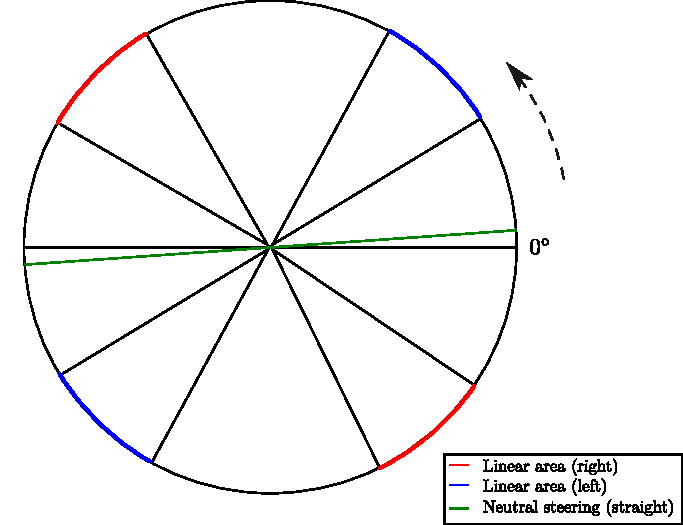
\includegraphics[width=0.8\textwidth]{figures/servoSteeringLinearArea.pdf}
  \caption{A representation of the servomotor's angle positions with the steering linear areas}
  \label{fig:servoSteeringLinearArea}
\end{figure}

The diameters on the circle represent the servo arm which spins around a central position. The green line, shifted of a few degrees from the \si{0^{\circ}} is the position allowing the vehicle to go straight. The linear areas of steering are represented by the red and blue arcs : to turn to the left, the servo angle has to be increased as well as the pulse width.

Still due to mechanical imperfections on the vehicle, the offset that has to be applied to the servo pulse width to reach the linear area for steering is different depending on which way the vehicle is turning. It also varies a bit with the ground texture it is running on because of the friction it offers and it thus has to be tuned accordingly.
The actual value of this offset is empirically found to be close to \si{\pm 250\ ms}.\\
%
Moreover, the actual pulse width value which allows the vehicle to run straight is not the same that sets the servomotor to its middle position and may slightly vary through time because of mechanical wear.